\chapter{Exercise 04}
\extitle{Multivariate Gradient Descent}
%******************************************************************************%
%                                                                              %
%                                 Interlude                                    %
%                         for Machine Learning module                          %
%                                                                              %
%******************************************************************************%

% =============================================== %
\section*{Interlude - Regularized Gradient}
% =============================================== %
\begin{figure}[!h]
    \centering
    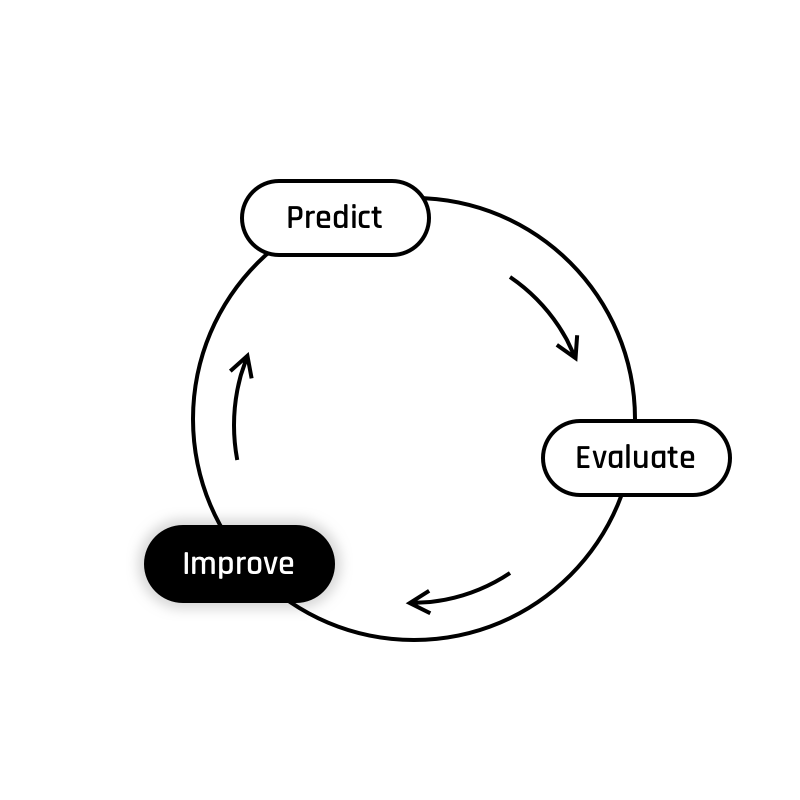
\includegraphics[scale=0.25]{assets/Improve.png}
    %\caption{The Learning Cycle: Improve}
\end{figure}
\noindent{To derive the gradient of the regularized loss function, $\nabla(J)$ 
you have to change a bit the formula of the unregularized gradient.}\\
\\
Given the fact that we are not penalizing $\theta_0$, the formula will remain 
the same as before for this parameter. For the other parameters ($\theta_1, \dots, \theta_n$),
 we must add the partial derivative of the regularization term: $\lambda \theta_j$.\\
\\
Therefore, we get:
$$
\nabla(J)_0 = \frac{1}{m}\sum_{i=1}^{m}(h_\theta(x^{(i)}) - y^{(i)})
$$
$$
\nabla(J)_j = \frac{1}{m}\left(\sum_{i=1}^{m}(h_\theta(x^{(i)}) - y^{(i)})x_j^{(i)} + \lambda \theta_j\right) \text{ for j = 1, ..., n}
$$
\\
Where:  
\begin{itemize}
    \item $\nabla(J)_j$ is the j$^\text{th}$ component of the gradient vector $\nabla(J)$
    \item $m$ is the number of training examples used
    \item $h_\theta(x^{(i)})$ is the model's prediction for the i$^\text{th}$ training example
    \item $x^{(i)}$ is the feature vector of the i$^\text{th}$ training example
    \item $y^{(i)}$ is the expected target value for the i$^\text{th}$ example
    \item $\lambda$ is a constant, the regularization hyperparameter
    \item $\theta_j$ is the j$^\text{th}$ parameter of the $\theta$ vector
\end{itemize}
\bigskip
Which can be vectorized as:
$$
\nabla(J) = \frac{1}{m} [X'^T(h_\theta(X) - y) + \lambda \theta']
$$  
\\
Where:  
\begin{itemize}
    \item $\nabla(J)$ is a vector of length $(n + 1)$, the gradient vector
    \item $m$ is the number of training examples used
    \item $X$ is a matrix of dimension $(m \times n)$, the design matrix
    \item $X'$ is a matrix of dimension $(m \times (n + 1))$, the design matrix onto 
    which a column of ones is added as a first column
    \item $y$ is a vector of length $m$, the vector of expected values
    \item $h_\theta(X)$ is a vector of length $m$, the vector of predicted values
    \item $\lambda$ is a constant
    \item $\theta$ is a vector of length $(n + 1)$, the parameter vector
    \item $\theta'$ is a vector of length $(n + 1)$, constructed using the following rules:
\end{itemize}

$$
\begin{matrix}
\theta'_0 & =  0 \\
\theta'_j & =  \theta_j & \text{ for } j = 1, \dots, n\\    
\end{matrix}
$$

% =============================================== %
\subsection*{Linear Gradient vs Logistic Gradient}
% ----------------------------------------------- %
As before, we draw your attention on the only difference between the linear regression's 
and the logistic regression's gradient equations: \textbf{the hypothesis function} $h_\theta(X)$.
\begin{itemize}
    \item In the linear regression: $h_\theta(X) = X'\theta$
    \item In the logistic regression: $h_\theta(X) = \text{sigmoid}(X'\theta)$
\end{itemize}

\newpage
\turnindir{ex04}
\exnumber{04}
\exfiles{fit.py}
\exforbidden{any function that performs derivatives for you}
\makeheaderfilesforbidden


% ================================= %
\section*{Objective}
% --------------------------------- %
Understand and manipulate the concept of gradient descent in the case of multivariate linear regression.\\
\newline
Implement a function to perform linear gradient descent (LGD) for multivariate linear regression.

% ================================= %
\section*{Instructions}
% --------------------------------- %
In this exercise, you will implement linear gradient descent to fit your multivariate model to the dataset.\\
\newline
The pseudocode of the algorithm is the following:

$$
\begin{matrix}
    &   \text{repeat until convergence} \hspace{1cm} &  \{  \\
    &   \text{compute } \nabla{(J)}  \\
    &	\theta := \theta - \alpha \nabla(J)                 \\ 
\} 
\end{matrix}
$$
Where:
\begin{itemize}
  \item $\nabla{(J)}$ is the entire gradient vector
  \item $\theta$ is the entire parameter vector
  \item $\alpha$ (alpha) is the learning rate (a small number, usually between 0 and 1)
\end{itemize}
% ================================= %
\newpage
\noindent{You are expected to write a function named \textit{fit\_} as per the instructions bellow:\\}
\newline
\begin{minted}[bgcolor=darcula-back,formatcom=\color{lightgrey},fontsize=\scriptsize]{python}
def fit_(x, y, theta, alpha, max_iter):
  """
  Description:
    Fits the model to the training dataset contained in x and y.
  Args:
    x: has to be a numpy.array, a matrix of dimension m * n:
                  (number of training examples, number of features).
    y: has to be a numpy.array, a vector of dimension m * 1:
                  (number of training examples, 1).
    theta: has to be a numpy.array, a vector of dimension (n + 1) * 1:
                  (number of features + 1, 1).
    alpha: has to be a float, the learning rate
    max_iter: has to be an int, the number of iterations done during the gradient descent
  Return:
    new_theta: numpy.array, a vector of dimension (number of features + 1, 1).
    None if there is a matching dimension problem.
    None if x, y, theta, alpha or max_iter is not of expected type.
  Raises:
    This function should not raise any Exception.
  """
    ... your code here ...
\end{minted}
\\
Hopefully, you have already implemented a function to calculate the multivariate gradient.
% ================================= %
\section*{Examples}
% ================================= %
\begin{minted}[bgcolor=darcula-back,formatcom=\color{lightgrey},fontsize=\scriptsize]{python}
import numpy as np
x = np.array([[0.2, 2., 20.], [0.4, 4., 40.], [0.6, 6., 60.], [0.8, 8., 80.]])
y = np.array([[19.6], [-2.8], [-25.2], [-47.6]])
theta = np.array([[42.], [1.], [1.], [1.]])

# Example 0:
theta2 = fit_(x, y, theta,  alpha = 0.0005, max_iter=42000)
theta2
# Output:
array([[41.99..],[0.97..], [0.77..], [-1.20..]])

# Example 1:
predict_(x, theta2)
# Output:
array([[19.5992..], [-2.8003..], [-25.1999..], [-47.5996..]])
\end{minted}

\info{
  \begin{itemize}
    \item You can create more training data by generating an $x$ array with random values and computing the corresponding $y$ vector as a linear expression of $x$.
          You can then fit a model on this artificial data and find out if it comes out with the same $\theta$ coefficients that first you used.
    \item It is possible that $\theta_0$ and $\theta_1$ become \texttt{"nan"}.
          In that case, it means you probably used a learning rate that is too large.
  \end{itemize}
}